
\begin{flushleft}
	\begin{itemize}
		\item If you’re coming from Windows, you must be aware of C: drive, D: drive etc.
		\item In Linux, there is \textbf{no} C: or D: drive. 
		\item Linux have standard directory structure called Filesystem Hierarchy Standard (FHS).
	\end{itemize}
	
	\begin{tcolorbox}[breakable,notitle,boxrule=-1pt,colback=yellow,colframe=yellow]
		\color{black}
		\bigskip
		Note: Folder and directory means the same!
		\bigskip
	\end{tcolorbox}
	
	\bigskip
	\begin{figure}[h!]
		\centering
		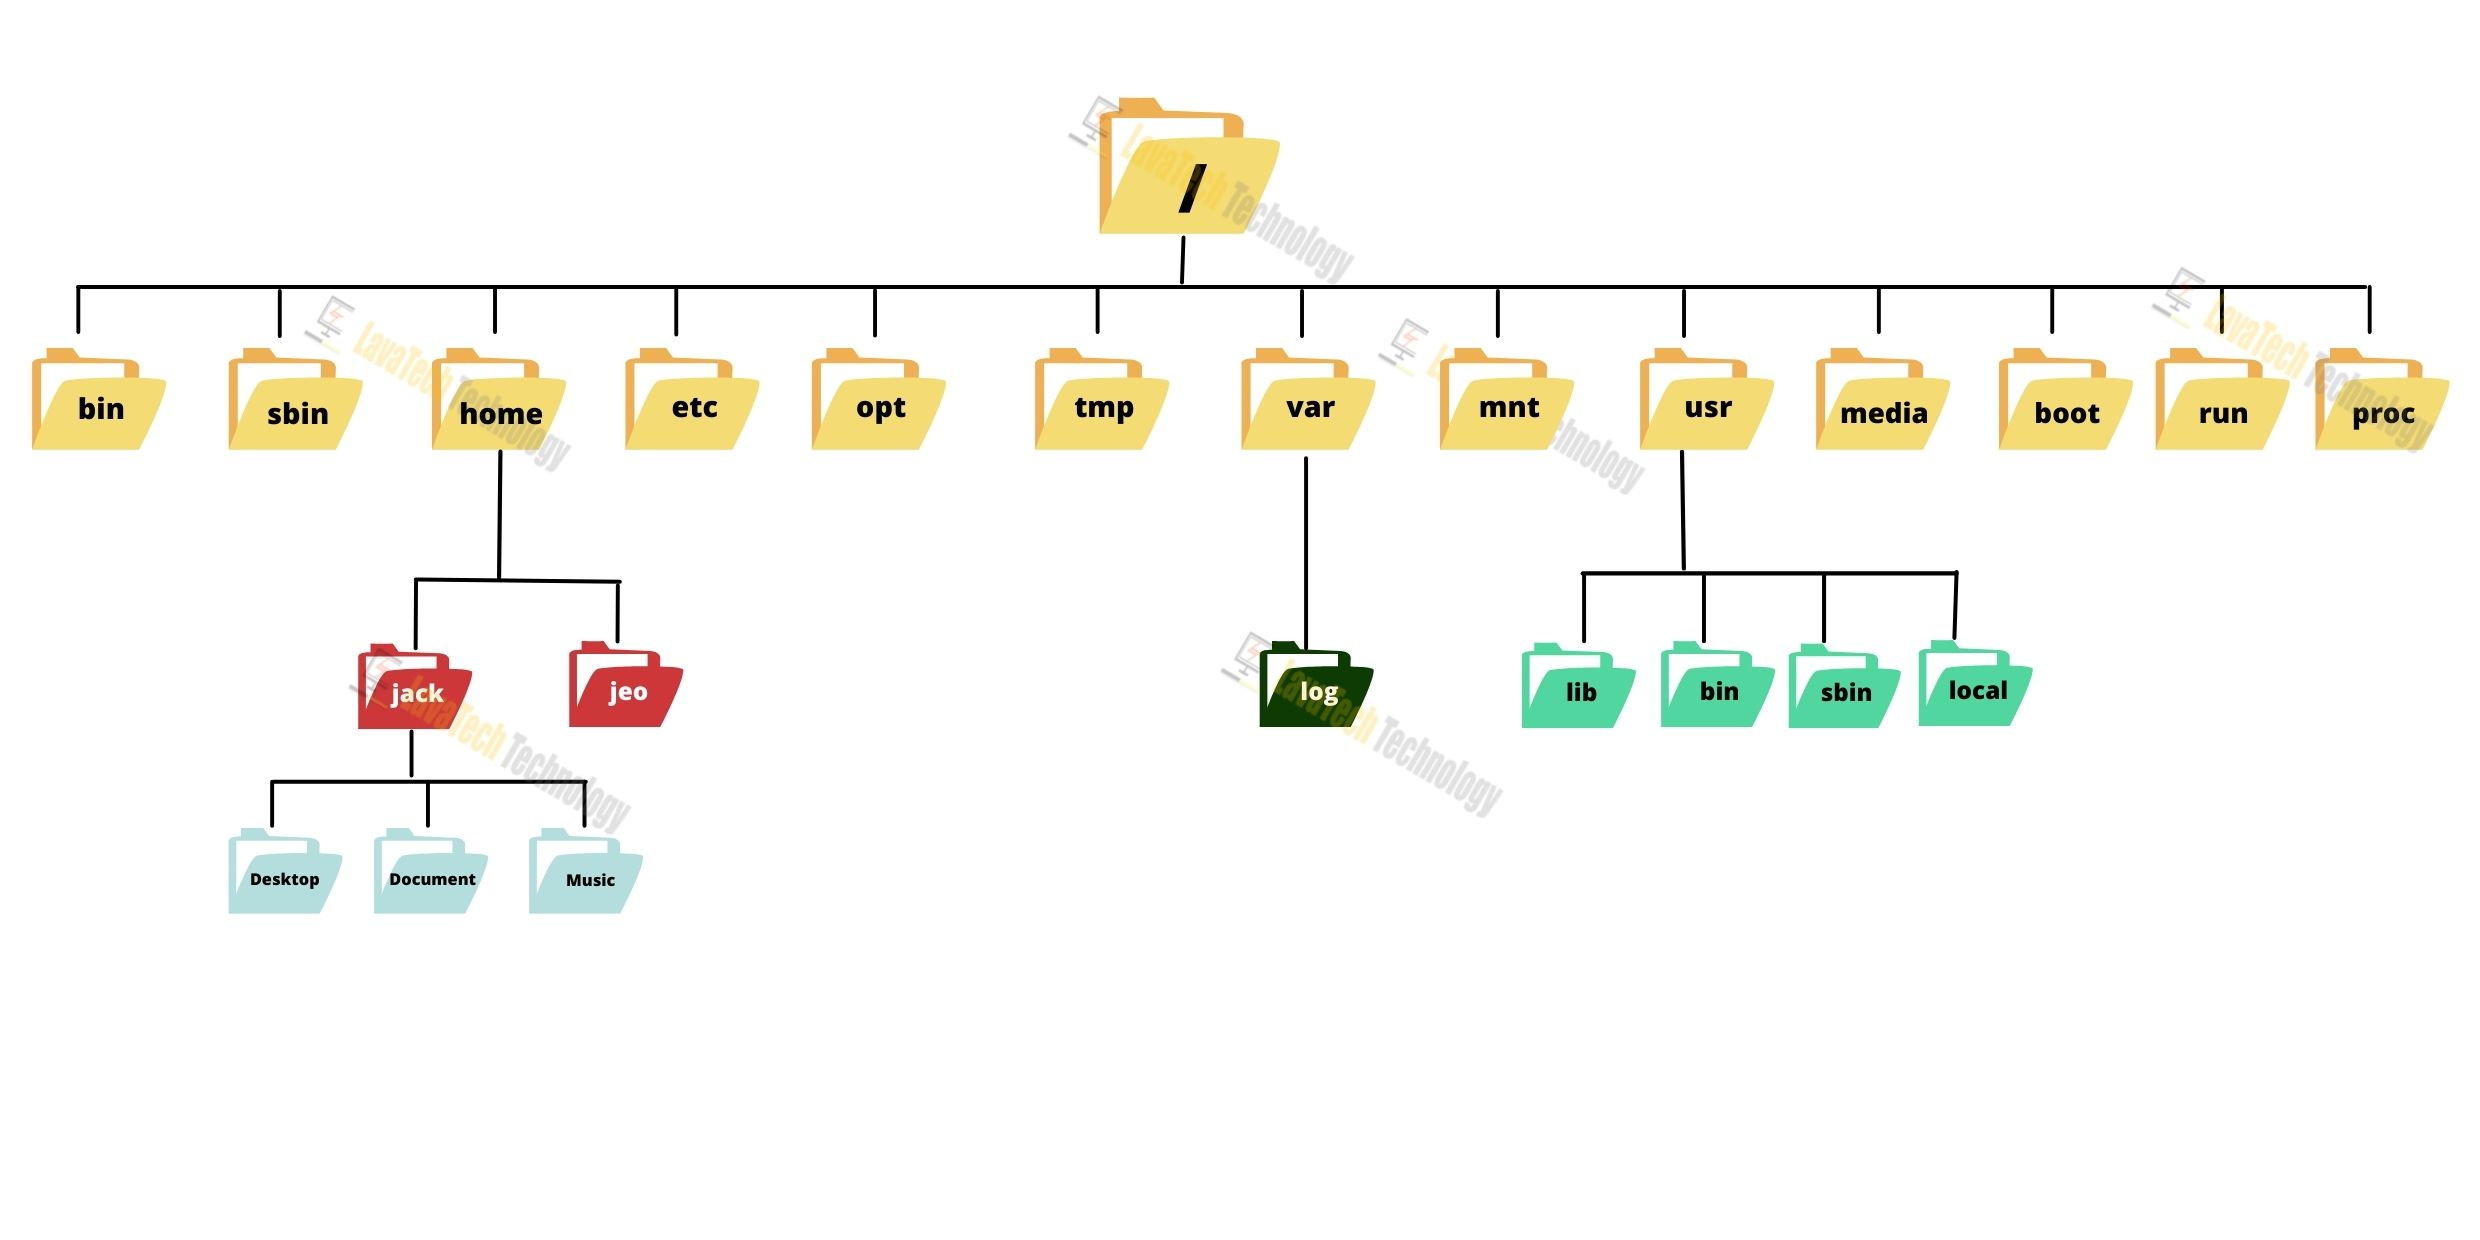
\includegraphics[scale=.24]{content/chapter2/images/fhs.jpg}
		\caption{Filesystem Hierarchy Standard (FHS)}
		\label{fig:fhs}
	\end{figure}
\end{flushleft}

\newpage

